\documentclass[12pt,oneside,openany,a4paper,%..... Layout
               afrikaans, english,%.............. Global language selection
               ]{memoir}

 \usepackage[masters-t,%.......................... Master thesis
             goldenblock,%........................ A5 type block (or a5block or wide)
            ]{usthesis}%.......................... US thesis style with memoir

%
% PLEASE read the USthesis documentation for the class options
% and how to set line and paragraph spacing
%

%==== Language setup ================================================
 \usepackage[latin1]{inputenc}%................... Recognizes �, �, etc
 \usepackage{babel}%.............................. Language setup

%==== Math setup ====================================================
 \usepackage{amsmath}%............................ Advanced math (before fonts)
 %\usepackage{amssymb}%............................ AMS Symbol fonts

%==== Font setup (default is Computer Modern) =======================
 \usepackage[T1]{fontenc}%........................ Type 1 fonts
 %\usepackage{fourier}
 \usepackage{textcomp}%........................... Additional text character
 \usepackage{bm}%................................. Bold math symbols (after fonts)

%==== Ref's, Bib's and Nomencl ======================================
 \usepackage{usnomencl}%.......................... List of symbols (in usthesis pack)
 \usepackage{usbib}%.............................. Bibliography    (in usthesis pack)
    \bibliographystyle{usmeg-a}
    \renewcommand\bibfont{\small}

    %% For usmeg-a, the bib is a list of references. If you
    %% are using usmeg-n comment out the following lines
    \addto{\captionsafrikaans}{\renewcommand{\bibname}{Lys van Verwysings}}
    \addto{\captionsenglish}{\renewcommand{\bibname}{List of References}}

%==== Graphics and Color ============================================
\usepackage{graphicx}%........................... Graphicx loaded in usthesis
\usepackage{color}%.............................. Color setup
\usepackage{eso-pic}%............................ Shipout commands for watermark
    \newcommand*{\WaterMark}[2][0.15\paperwidth]{%
        \AddToShipoutPicture*{\AtTextCenter{%
                \parbox[c]{0pt}{\makebox[0pt][c]{%
                    \includegraphics[width=#1]{#2}}}}}}

%==== Local Defs ====================================================
\makeatletter

%
% Please insert user defined commands here
% and NOT in the document itself!
%

\makeatother

%==== TITLE PAGE ====================================================
\title{\bfseries
       \AorE{%-- Afrikaans ------------------------------------------
             Title\\[1ex]
             \normalfont\small\itshape
             (``Title'')
            }{%-- English -------------------------------------------
             Title
            }}

%\author{D.\ W.\ Wolsky}{David William Wolsky}
\author{A.}{Author}

\degree{\AorE{MIng (Elek)}{MEng (Elec)}}
       {\AorE{Magister in Ingenieurswese (Elektroniese )}
             {Master of Engineering (Electronic)}}

\address{\AorE{%-- Afrikaans ----------------------------------------
        Departement Elektriese en Elektroniese Ingenieurswese,\\
        Universiteit van Stellenbosch,\\
        Privaatsak X1, Matieland 7602, Suid Afrika.%
             }{%-- English ------------------------------------------
        Department of Electrical and Electronic Engineering,\\
        University of Stellenbosch,\\
        Private Bag X1, Matieland 7602, South Africa.
             }}

\faculty{\AorE{Fakulteit Ingenieurswese}%
              {Faculty of Engineering}}

%\supervisor{Prof.\ D.\ De Villiers}
\supervisor{Supervisor}
%\cosupervisor{Mnr.\ J.\ Smith}

\setdate{12}{2015}

%\SetSponsor{The financial assistance of the National Research Foundation (NRF)
%    towards this research is hereby acknowledged. Opinions expressed and
%    conclusions arrived at, are those of the author and are not necessarily to
%    be attributed to the NRF.}


%====================================================================
%     MAIN DOCUMENT
%====================================================================
\maxsecnumdepth{subsubsection}
\maxtocdepth{section}

\begin{document}

%==== Front matter ==================================================
 \frontmatter
 \WaterMark{UScrest-WM}
 \TitlePage

% \DeclarationDate{\today}
 \DeclarationDate{date}
 \DeclarationPage

 \begin{abstract}[english]%===================================================
abstract
\end{abstract}


\begin{abstract}[afrikaans]%=================================================
abstrakte
\end{abstract}


\chapter{Acknowledgements}%==================================================

I would like to express my sincere gratitude to the following people
and organisations ...


\chapter{Dedications}%=======================================================
 \vfill
 \begin{Afr}
 \begin{center}\itshape
    Hierdie tesis word opgedra aan ...
 \end{center}
 \end{Afr}
 \vfill
 \clearpage

%============================================================================
\endinput


 \tableofcontents
 \clearpage

 \setcounter{lofdepth}{2}
 \listoffigures
 \clearpage

 \listoftables
 \clearpage

 \chapter{Nomenclature}

\begin{Nomencl}
 \NomGroup{Constants}%-----------------------------------------------
   \item[$\mathrm{g} = $] $\mathrm{9.81\,m/s^2}$

 \NomGroup{Variables}%-----------------------------------------------
   \item[$\mathit{Re}_\mathrm{\,D}$]
                      \UnitLine{Reynolds number (diameter)}{~}
   \item[$x$]         \UnitLine{Coordinate                }{m}
   \item[$\ddot{x}$]  \UnitLine{Acceleration              }{m/s^2}\\
   \item[$\theta$]    \UnitLine{Rotation angle            }{rad}
   \item[$\tau$]      \UnitLine{Moment                    }{N{\cdot}m}

 \NomGroup{Vectors and Tensors}%-------------------------------------
   \item[$\overrightarrow{\bm{v}}$] Physical vector, see equation ...

 \NomGroup{Subscripts}%----------------------------------------------
   \item[$\mathrm{a}$] Adiabatic
   \item[$a$]          Coordinate
\end{Nomencl}



\endinput


%==== Main document =================================================
\mainmatter
   \setsecnumdepth{subsubsection}
%   \numberwithin{equation}{section}
%   \numberwithin{figure}{chapter}
%   \numberwithin{table}{chapter}

\chapter{Discrete Element Method}
\label{chp:DEM}


%%%%%%%%%%%%%%%%%%%%%%%%%%%%%%%%%%%%%%%%%%%%%%%%%%%%%%%%%%%%%%%%%%%%%%%
\section{Introduction}

Introduction...
%TODO
\chapter{Literature review}
\label{chp:LitReview}

%%%%%%%%%%%%%%%%%%%%%%%%%%%%%%%%%%%%%%%%%%%%%%%%%%%%%%%%%%%%%%%%%%%%%%%
\section*{Process}
%TODO remove this
\begin{itemize}
\item Keep problem statement in the foremost of the author's mind: \\ \textit{Trust region use with SM for particular antenna design}.
\item Obtain reference material and understand it.
\item Organise texts.
\item Document relevant material using paragraphs in your own words citing references.
\end{itemize}

%%%%%%%%%%%%%%%%%%%%%%%%%%%%%%%%%%%%%%%%%%%%%%%%%%%%%%%%%%%%%%%%%%%%%%%
\section{Optimisation}
Describe the different optimisation problems that are required in a typical or subset of antenna design processes.

%%%%%%%%%%%%%%%%%%%%%%%%%%%%%%%%%%%%%%%%%%%%%%%%%%%%%%%%%%%%%%%%%%%%%%%
\section{Space mapping}
%TODO put into actual paragrpah
Introduction to what SM is and discuss the different types. Explain the basic SM techniques roughly and what they work for, details to follow. Problem is that they require a highly complex surrogate model. There are also more advanced algorithms that only require simple surrogate models. GSM, FDGSM.
\subsection{Implicit space mapping (ISM)}
\subsection{Output space mapping (OSP)}
\subsection{Space mapping interpolating surrogates (SMISs)}
\subsection{Generalised space mapping (GSM)}
\subsection{Frequency-dependent generalised space mapping (FDGSM)}
Space mapping

%TODO the objective of the literature servery is to obtain material that supports the work at hand. 


%%%%%%%%%%%%%%%%%%%%%%%%%%%%%%%%%%%%%%%%%%%%%%%%%%%%%%%%%%%%%%%%%%%%%%%
\section{Actual paper summaries}
%TODO so this somewhere else like where Andries mentioned 
\subsection{A Space-Mapping Framework for Engineering Optimisation - Theory and Implementation: Koziel, Bandler and Madsen \cite{SMFrameworkKoziel} }
\subsubsection*{Introduction and background}
Space-mapping (SM) is a widely used engineering optimisation paradigm [citations].
SM uses two different models to run an optimisation on. The one model is a fine model that is a very good approximation of the `real world' model. This is computationally expensive to run and a surrogate or coarse model is used that is cheaper to evaluate. There is a misalignment between these two models, but if they are still fairly good representation of the `real world' model the misalignment should be small. If the alignment is indeed good then SM-based optimisation algorithms typically provide good results with few evaluations of the computationally expensive fine model. 
\\ \\
SM is used extensively for models at microwave frequencies. The full-wave electromagnetic (EM) solvers take a long time to run [validate with own examples/citations if for own use], but they can be represented by physical based equivalent-circuit models that are cheap to simulate. 
\\ \\
There are other engineering disciplines that have started using SM techniques. Bandler review [5](Bandler, Cheng, Dakroury, Mohamed, Bakr, Madsen and Sondergaard; Space mapping: the state of the art).
\\ \\
Mentioned SM techniques with references:\\
Implicit space mapping (ISM)\\
Output space mapping (OSP)\\
Space mapping interpolating surrogates (SMISs)\\
Generalised space mapping (GSM)\\
Frequency-dependent generalised space mapping (FDGSM)\\
\\ \\
The actual paper describes algorithms that exploit surrogate models based on OSM that force exact matching of responses and Jacobians between the fine and the surrogate model. Theoretical results are presented that show the influence of Jacobian matching on the convergence of the optimisation algorithm. Design-variable-dependent ISM is introduced to increase the flexibility of the surrogate model in a consistent way. Also proposed to make more accessible to engineers using particular tools. 
\\ \\
Engineering design optimisation exploiting SM. \\
GISM to minimise misalignment between fine and course models.\\
Output SM to ensure the matching of response and first-order derivatives between mapped coarse and fine models at the current iteration point in the optimisation process.\\

\subsubsection*{Surrogate Optimisation}
The optimisation problem is seen in Equation \ref{eqn:optimisationProblem}
\begin{equation}
\textbf{R}_f : X_f \rightarrow R^m \underline{\subset} R^n
\label{eqn:optimisationProblem}
\end{equation}
Where: \\
$\textbf{R}_f$ is the response vector of the fine model. For example in microwave systems it could be the model evaluation of the scattering parameter $|S_{12}|$. \\
$m$ in the subscript of $R_m$ represents the number of different frequency points. \\
The goal of the optimisation is to solve 
\begin{equation}
\textbf{\textit{x}}^{*}_f = \mathrm{arg} \, \underset{\textbf{\textit{x}} \epsilon X_{f}}{\mathrm{min}} \, U \, ( \textbf{R}_{\textbf{f}} (\textbf{\textit{x}}) ) 
\label{eqn:optimisationGoal}
\end{equation}
where $U$ is the objective function. It is assumed that the fine model is too computationally expensive to solve directly using the fine model. Instead inexpensive surrogate models are used. These are not as accurate as the fine model but are computationally cheap, which allows them to be run many times. An optimisation algorithms that generates a sequence of points $\textbf{\textit{x}}^{(i)} \, \epsilon \, X_f, i = 1,2,\cdots $ and a family of surrogate models 
\begin{equation}
\textbf{R}_s^{(i)} \, : \, X_s^{(i)} \rightarrow R^m, i=0,1,\cdots" 
\end{equation}
so that 
\begin{equation}
\textbf{\textit{x}}^{(i+1)} = \mathrm{arg} \, \underset{\textbf{\textit{x}} \epsilon X_s^{(i)} \cap X_f}{\mathrm{min}} \, U \, \left(\textbf{R}^{(i)}_s (\textbf{\textit{x}})\right)
\end{equation}
and $\textbf{R}_s^{(i+1)}$ is constructed using a suitable matching condition with the fine model at previous point $\textbf{\textit{x}}^{(k)}, k=1,\cdots,i$. 
\\ \\
SM uses that assumption that there is a coarse model $\textbf{R}_c : X_c \rightarrow R^m, X_c \underline{\subset} R^n$ that describes the same object as the fine model. A family of surrogate models is built up of a suitable distribution of $\textbf{R}_c$ such that matching conditions are satisfied. 
%TODO what exactly is meant by matching conditions in this context.

%TODO --- --- --- --- --- --- --- --- ---
%TODO --- --- ---  here i am  --- --- ---
%TODO --- --- --- --- --- --- --- --- ---


\subsubsection*{Generalised Implicit Space-Mapping (GISM)}
Enhancement of \textit{Space Mapping Optimization Algorithms for Engineering Design,
Koziel 2006}, \cite{SMOptAlgEngDesignKoziel}, using design-variable dependent ISM.Also recall \textit{Implicit Space Mapping Optimization Exploiting Preassigned Parameters, Bandler 2004}, \cite{ImplicitSMExploitParametersBandler}.
Using a coarse model that depends on preassigned parameters,
$$
\textbf{R}_c \, : \, X_c \times X_p \rightarrow R^m
$$
where $X_p \,\underline{\subset} \, R^q$ is a domain with preassigned parameters. \\
\\
The ISM optimisation algorithm adjusts the preassigned parameters $\textbf{\textit{x}}_p$ so that, at the current point $\textbf{\textit{x}}^{(i)}$, the both the fine model and the coarse model response vectors match. The adjustment can be referred to as a preadjustment  and that adjusted model becomes a surrogate. This in turn is used to obtain the next point $\textbf{\textit{x}}^{(i+1)}$. 

\begin{equation}
\textbf{R}_s^{(i)}(\textbf{\textit{x}}) = 
\textbf{R}_c \left( \textbf{\textit{x}}^{(i)}_p, \textbf{\textit{x}} \right)
\label{eqn:surrogate}
\end{equation}

where $\textbf{\textit{x}}^{(i)}_p$ is determines by solving the parameter-extraction problem of the for 

\begin{equation}
\textbf{\textit{x}}^{(i)}_p = 
\textup{arg} \, \underset{\textbf{\textit{x}}}{\textup{min}} 
\vert\vert
\textbf{R}_f \left( \textbf{\textit{x}}^{(i)} \right) - 
\textbf{R}_c \left(  \textbf{\textit{x}}^{(i)}, \textbf{\textit{x}} \right)
\vert\vert
\end{equation}

Making preassigned parameters depend on design variables allows the number of degrees of freedom in the surrogate model \ref{eqn:surrogate} to be increased. In particular,
\begin{equation}
\textbf{R}_s^{(i)}(\textbf{\textit{x}}) = 
\textbf{R}_c \left( \textbf{\textit{x}}, \textbf{G}^{(i)}\textbf{\textit{x}} + \textbf{\textit{x}}^{(i)}_p \right)
\end{equation}
where $ \textbf{G}^{(i)} \, \epsilon \, M_{q \times n} $ and $ \textbf{\textit{x}}^{(i)}_p $ are determined by solving the parameter-extraction problem 
\begin{equation}
\left( \textbf{G}^{(i)},\textbf{\textit{x}}^{(i)}_p \right) = 
\textup{arg} \, \underset{(\textbf{G,\textit{x}})}{\textup{min}} 
\vert\vert
\textbf{R}_f \left( \textbf{\textit{x}}^{(i)} \right) - 
\textbf{R}_f \left(  \textbf{\textit{x}}^{(i)}, \textbf{G} \cdot  \textbf{\textit{x}}^{(i)} + \textbf{\textit{x}} \right) 
\vert\vert
\end{equation}

Combining this with the GSM from \cite{SMOptAlgEngDesignKoziel}, a GISM framework can be defined with the family of surrogate models $\textbf{R}^{(i)}_s$ defined as
\begin{equation}
\textbf{R}^{(i)}_s(\textbf{\textit{x}}) 
= \textbf{A}^{(i)} \cdot \textbf{R}_c
\left( \textbf{B}^{(i)}\cdot\textbf{\textit{x}} + \textbf{c}^{(i)} , \textbf{G}\cdot\textbf{\textit{x}} + \textbf{\textit{x}}^{(i)}_p \right) + 
\textbf{d}^{(i)} + \textbf{E}^{(i)} \cdot \left( \textbf{\textit{x}} - \textbf{\textit{x}}^{(i)} \right)
\end{equation}
where 
\begin{equation}
\left( \textbf{A}^{(i)}, \textbf{B}^{(i)}, \textbf{c}^{(i)}, \textbf{G}^{(i)}, \textbf{\textit{x}}^{(i)}_p \right) = 
\textup{arg} \, \underset{(\textbf{A},\textbf{B},\textbf{c},\textbf{G},\textbf{\textit{x}}_p)}{\textup{min}} 
\varepsilon^{(i)}(\textbf{A},\textbf{B},\textbf{c},\textbf{G},\textbf{\textit{x}}_p)
\end{equation}

\begin{equation}
\textbf{d}^{(i)} = \textbf{R}_f \left( \textbf{\textit{x}}^{(i)} \right) - 
\textbf{A}^{(i)} \textbf{R}_c
\left(
     \textbf{B}^{(i)} \cdot  \textbf{\textit{x}}^{(i)} + \textbf{c}^{(i)},
     \textbf{G}^{(i)} \cdot \textbf{\textit{x}} + \textbf{\textit{x}}^{(i)}_p
\right)
\label{eqn:d}
\end{equation}

\begin{multline}
\textbf{E}^{(i)} = \textbf{J}_{\textbf{R}_f} \left( \textbf{\textit{x}}^{(i)} \right) 
- 
\textbf{A}^{(i)} \cdot \textbf{J}_{\textbf{R}_c \cdot \textbf{\textit{x}}}
    \left(
        \textbf{B}^{(i)} \cdot \textbf{\textit{x}}^{(i)} + \textbf{c}^{(i)},
        \textbf{G}^{(i)} \cdot \textbf{\textit{x}} + \textbf{\textit{x}}^{(i)}_p
    \right) \cdot \textbf{B}^{(i)} 
\\ -
\textbf{A}^{(i)} \cdot \textbf{J}_{\textbf{R}_c \cdot \textbf{\textit{x}}_p}
    \left(
        \textbf{B}^{(i)} \cdot \textbf{\textit{x}}^{(i)} + \textbf{c}^{(i)},
        \textbf{G}^{(i)} \cdot \textbf{\textit{x}} + \textbf{\textit{x}}^{(i)}_p
    \right) \cdot \textbf{G}^{(i)}
\label{eqn:E}
\end{multline}

From the above the following matrices 
$$
\textbf{A}^{(i)} = diag\{ a^{(i)}_1, \cdots , a ^{(i)}_m \}
$$
$$
\textbf{B}^{(i)} \, \epsilon \, \textup{M}_{n \times n}
$$
$$
\textbf{c}^{(i)} \, \epsilon \, \textup{M}_{n \times 1}
$$
$$
\textbf{G}^{(i)} \, \epsilon \textup{M}_{q \times n}
$$
as well as vector $\textbf{\textit{x}}^{(i)}_p$ are found using parameter extraction applied to the matching condition $\varepsilon ^{(i)}$. \\
Matrices 
$$
\textbf{d}^{(i)} \, \epsilon \, \textup{M}_{m \times 1}
$$
and 
$$
\textbf{E}^{(i)} \, \epsilon \, \textup{M}_{m \times n}
$$
are calculated using \ref{eqn:d} and \ref{eqn:E} respectively. $\textbf{J}_{\textbf{R}_c \cdot \textbf{\textit{x}}}$ and $\textbf{J}_{\textbf{R}_c \cdot \textbf{\textit{x}}_p}$ 
represent the Jacobian of the coarse model with respect to $\textbf{\textit{x}}^{(i)}$ and $\textbf{\textit{x}}^{(i)}_p$ respectively. 
\\ \\
The Jacobian is not always available [should site this and explain why solvers do not typically expose this] because it is expensive to calculate and not often exposed by full wave solvers ??
%TODO find this out...  
If the Jacobian information is not available, matrix $E^{(i)}$ can be estimated, for example, using the Broyden update. 
\\ \\
%TODO insert big section on what this is and what other estimates can be used.
\textit{Wiki - quasi-Newton method for finding roots. The idea is to compute the whole Jacobian only at the first iteration and to do rank-one update at the other iterations. This may not converge for non-linear systems.}
\\ \\
Form of matching condition and description of $w_k$ and $v_k$. Describes how the surrogate tries to match the fine model response at all previous $\textbf{\textit{x}}^{(k)}$ (including current point), but Jacobian matching is not exploited.
\\ \\
Input SM determined by matrices $ \textbf{B}^{(i)} $ and $ \textbf{c}^{(i)} $, the multiplication matrix $ \textbf{A}^{(i)} $, as well as the ISM parameters $ \textbf{\textit{x}}^{(i)}_p $ and  $ \textbf{G}^{(i)} $, can be considered as preconditioning of the coarse model that reduces the initial misalignment between the coarse and fine models over the neighbourhood of the current point $ \textbf{\textit{x}}^{(i)} $. 
\\
The terms $ \textbf{d}^{(i)} $ ensures perfect matching of responses at $ \textbf{\textit{x}}^{(i)} $ (zero order consistency). $ \textbf{E}^{(i)} $ gives perfect matching of first-order derivatives at $ \textbf{\textit{x}}^{(i)} $




\subsubsection*{Examples}
\begin{enumerate}
\item Bandpass filter
\item Bandpass filter with double-coupled resonators
\item Seven-section impedance transformer
\end{enumerate}
\subsubsection*{Conclusion}


%\chapter{Literature review}
\label{chp:DEM}


%%%%%%%%%%%%%%%%%%%%%%%%%%%%%%%%%%%%%%%%%%%%%%%%%%%%%%%%%%%%%%%%%%%%%%%
\section{Next Chapter}

Space mapping


%==== Appendices ====================================================
\appendix
\appendixpage\relax

\chapter{Discrete Element Method Theory}
\label{chp:DEM-Theory}

\section{Ball elements}
\label{sec:Ball-elems}

\begin{figure}
   \centering
   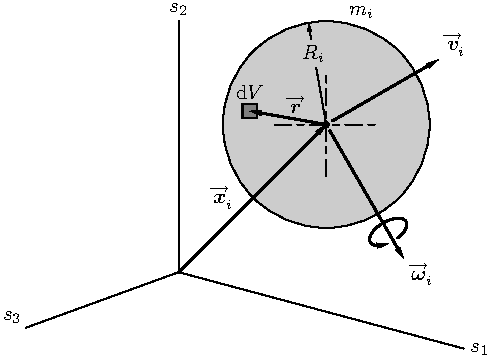
\includegraphics{figs/DEM-Def-Ball}
   \caption{Ball Element Parameters}
   \label{fig:BallDef}
\end{figure}


\subsection{Ball mass and inertia parameters}

Consider a volume element $\mathrm{d}V$ with respect to a static base $S$ of
an arbitrary solid body with  density $\rho$. The mass of the body is
obtained by integrating over the volume of the body,
\begin{equation}
    m = \int\limits_{\mathrm{body}} \rho\, \mathrm{d}V
    \label{eq:BMass-dif}
\end{equation}

In figure~\ref{fig:BallDef}, a ball with radius $R_{i}$ and uniform density
$\rho_i$ is depicted. The mass of the ball is after integration of
equation~\eqref{eq:BMass-dif}
\begin{equation}
    m_i = \tfrac{4}{3} \pi \rho_i\, R_i^3 .
    \label{eq:BMass}
\end{equation}


%----------------------------------------------------------------------------
\endinput

\chapter{Activity Log}
\label{chp:ActivityLog}

\section{Matlab}
\label{sec:ActivityLog-Matlab}

\subsection{Parameter sweep}
Recover lost work and get Windows machine up and running.\\
\begin{itemize}
\item 2016-01-22\\
Get back into the code and work out what is next.
\item 2016-01-20\\
Add gradient for parameter space iterations for multiple frequencies.\\
Problems with CADFEKO parameter sweep script -> log bug or follow up.\\
Validating responses, doesn't look right.
\item 2016-01-29\\
Add 3D plots. Add FEKO path to matlab so it runs correctly. \\
\item 2016-01-30\\
Visually validate $S_{11}$ results and of gradient w.r.t. parameter space.\\
\textcolor{red}{Problem}: Gradient seems to go bad after the first point.
\end{itemize}


\subsection{Tex}
\begin{itemize}
\item 2016-01-20\\
Create an activity log.
\item 2016-01-31\\
Describe how the gradient here links up with the Broyden update and in turn into $E^{(i)}$.
\end{itemize}
%----------------------------------------------------------------------------
\endinput

%\include{contents/App-3}

%==== Bibliography acro's & Index ===================================
\backmatter

\bibliography{backmatter/USbib-sample}

\end{document}
